\section{Reference surfaces and coordinate systems}
\label{Sect:RefSurf&CoordSysts}

\subsection{Doublet layer}
\label{SubSect:RefCoordDoublet}

The doublet-layer reference surface is defined to be the flat plane that is tangential to the outer surface of the mylar plane as shown in Figure \ref{Fig:DblLyrRef&Coord}a. The measured coordinate, $\alpha \in {u, v, w}$, is defined to lie in this plane and the $\alpha$ axis is perpendicular to the direction in which the fibres run. The doublet-layer $z_d$ axis is defined to to be perpendicular to the doublet-layer reference surface increasing in the direction indicated in the figure. The direction in which the measured coordinate, $\alpha$ increases is indicated in figure \ref{Fig:DblLyrRef&Coord}b. The orthogonal coordinate in the doublet-layer reference surface that with $\alpha$ and $z_d$ completes a right handed coordinate system is referred to as $\beta$. The $\beta$ axis is also indicated in figure \ref{Fig:DblLyrRef&Coord}b.

\begin{figure}
  \begin{center}
    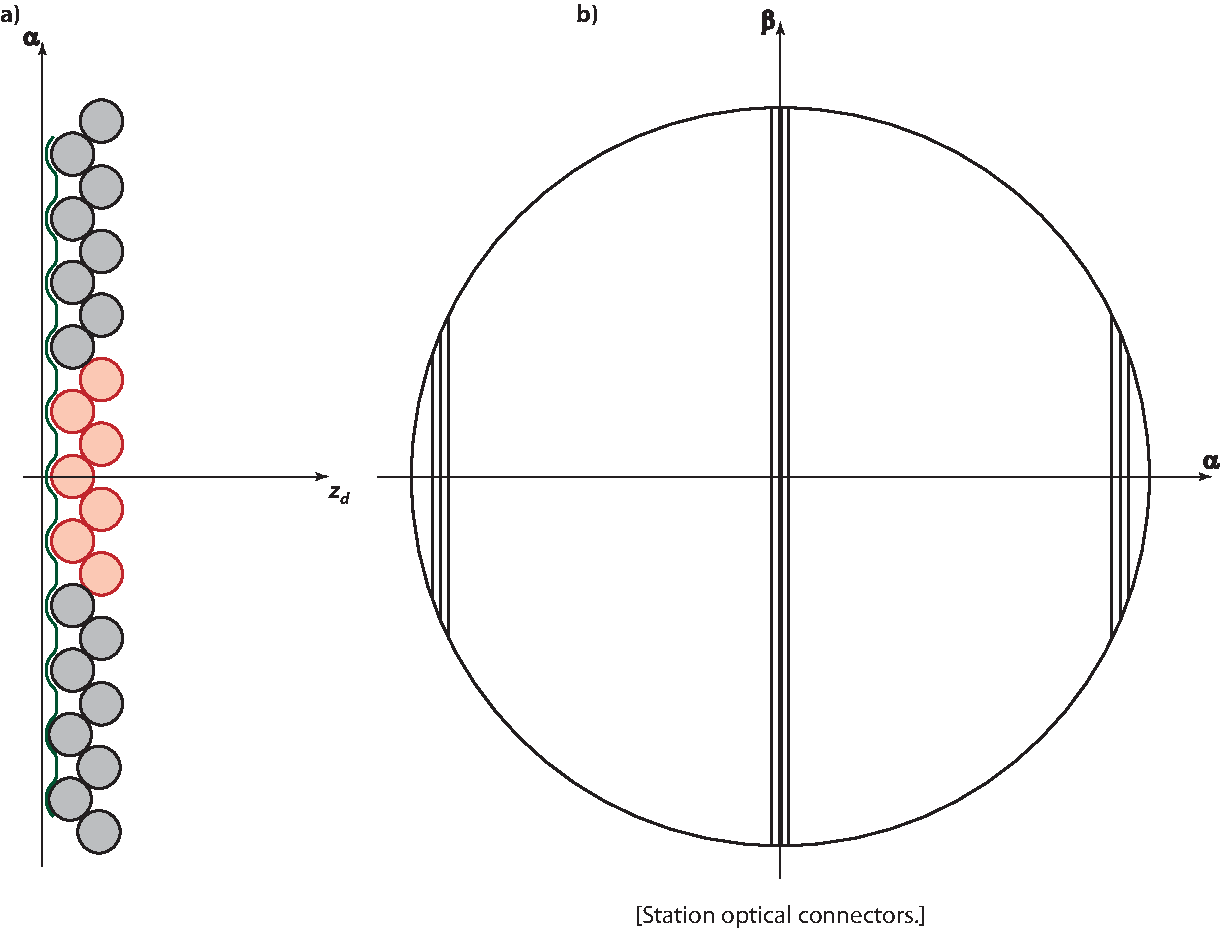
\includegraphics[width=0.7\linewidth] {detectors/tracker/03-Reference-surfaces-and-coordinate-systems/Figures/doublet-layer.pdf}
  \end{center}
  \caption{ Reference surfaces and coordinate-system definitions for the double layer and station. a) The fibres in the doublet layer are shown as the shaded circles, the central channel being shaded pink. The mylar layer is indicated by the solid black corrugated line. The doublet-layer reference surface is indicated by the vertical straight line, the arrow labelled $\alpha$ indicates the direction in which the coordinate measured by the doublet layer ($u$, $v$ or $w$) increases. The direction of the $z_d$ axis is indicated. b) View of doublet layer looking down on the mylar layer with the optical connectors at the bottom of the figure. The coordinate measured by the doublet layer ($u$, $v$ or $w$) is indicated by the axis labelled $\alpha$. The orthogonal axis, i.e. the direction in which the fibres run, is labelled $\beta$. The origin of the $(\alpha, \beta)$ coordinate system is taken to be at the centre of the circular active area.}
  \label{Fig:DblLyrRef&Coord}
\end{figure}

\subsection{Station}
\label{SubSect:RefCoordStn}

The station reference surface is defined to coincide with the reference surface of the $v$ doublet layer (see figure \ref{Fig:StnRef&Coord}). The station coordinate system is defined such that the $y_s$ axis is coincident with $v$ axis, the $z_s$ axis is coincident with the $z_d$ axis of the $v$ layer and the $x_s$ axis completes a right-handed coordinate system.

\begin{figure}
  \begin{center}
    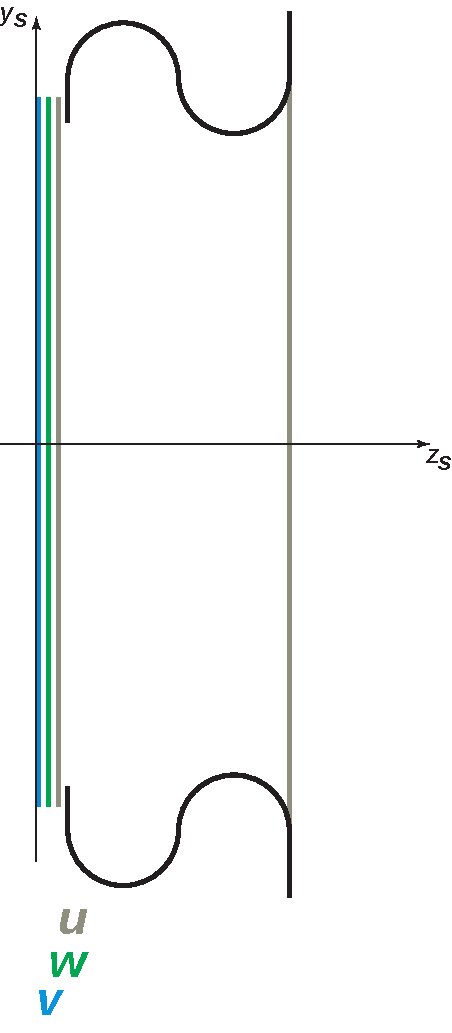
\includegraphics[width=0.22\linewidth]{detectors/tracker/03-Reference-surfaces-and-coordinate-systems/Figures/station.pdf}
  \end{center}
  \caption{ The carbon-fibre station body is indicated by the heavy solid black lines. The three doublet layers are indicated by the solid grey ($u$), green ($w$) and blue ($v$) lines. The station reference surface is shown by the solid vertical line coincident with the reference surface of the doublet layer labelled $v$. The direction $y_s$ axis, defined to be coincident with the $v$ axis and the $z_s$ axes are shown as the solid, black arrows. The $x_s$ axis completes a right-handed coordinate system and therefore points into the page. }
  \label{Fig:StnRef&Coord}
\end{figure}

\subsection{Tracker}
\label{SubSect:TrkrCoordStn}

The tracker reference surface is defined to coincide with the reference surface of station 1. The tracker coordinate system is defined such that the $z_t$ axis coincides with the nominal axis of cylindrical symmetry of the tracker as shown in figure \ref{Fig:TrkRef&Coord}. The tracker $z_t$ coordinate increases from station 1 to station 5. The tracker $y_t$ axis is defined to coincide with the $y_s$ axis of station 1 and the tracker $x_t$ axis completes a right-handed coordinate system.

\begin{figure}
  \begin{center}
    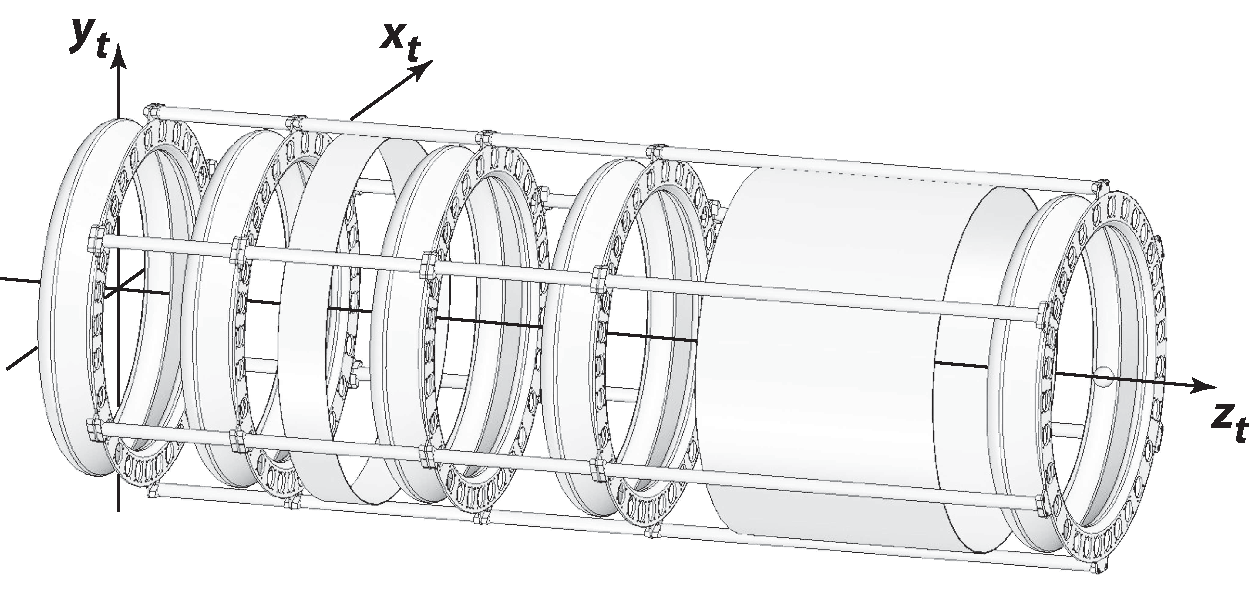
\includegraphics[width=0.7\linewidth]{detectors/tracker/03-Reference-surfaces-and-coordinate-systems/Figures/tracker.pdf}
  \end{center}
  \caption{ The outline of the components that make up the MICE tracker are shown in the line drawing. The tracker reference surface coincides with the reference surface of station 1. The tracker coordinate system is indicated by the solid lines. The $y_t$ axis is defined to be coincident with the $y_s$ axis in the station coordinate system.  The $z_t$ axis runs along the nominar axis of the tracker. The $x_t$ axis completes a right-handed coordinate system. }
  \label{Fig:TrkRef&Coord}
\end{figure}

\subsection{Coordinate transformations}
\label{SubSect:CoordTran}

\subsubsection{Doublet-layer to station}
\label{SubSubSect:DblStn}

The transformation from doublet-layer to station coordinates is achieved using the rotation $\underline{\underline{R}}_{SD}$ defined by: 

\begin{equation}
  {\bf r_s} = 
    \left(
        \begin{array}{c}
           x_s                                                      \\
           y_s
        \end{array}
    \right) = \underline{\underline{R}}_{SD} {\bf m} =
    \left(
        \begin{array}{cc}
           \cos \theta_D & -\sin \theta_D                           \\
           \sin \theta_D & -\cos \theta_D
        \end{array}
    \right) 
    \left(
        \begin{array}{c}
           \alpha                                                   \\
           \beta
        \end{array}
    \right) \, ;
\end{equation}
where $\theta_D$ is the angle which the fibres that make up the doublet-layer make to the $x_s$ axis in the station coordinate system.
